

\tikzset{every picture/.style={line width=0.75pt}} %set default line width to 0.75pt        

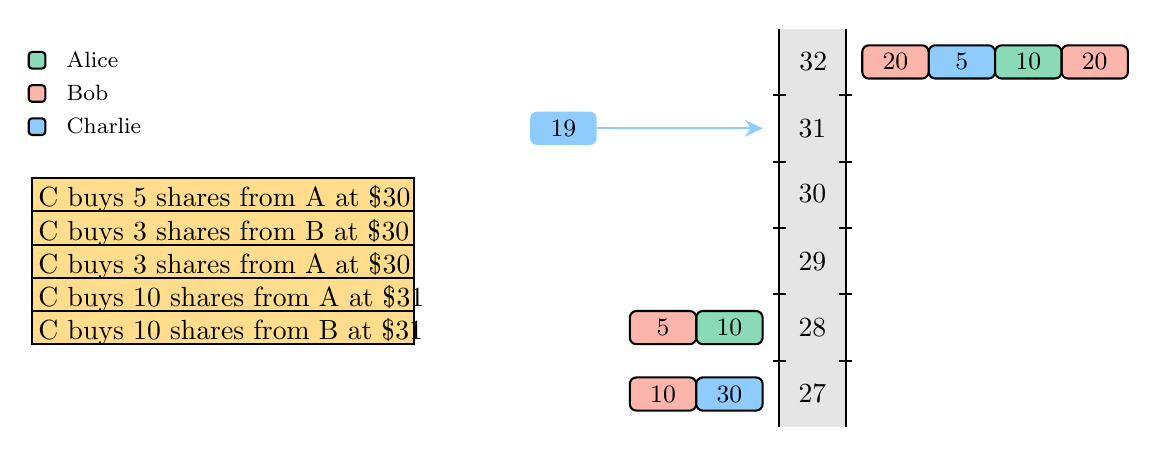
\begin{tikzpicture}[x=0.75pt,y=0.75pt,yscale=-0.8,xscale=0.8]
%uncomment if require: \path (0,300); %set diagram left start at 0, and has height of 300

%Shape: Rectangle [id:dp3861715993266832] 
\draw  [draw opacity=0][fill={rgb, 255:red, 0; green, 0; blue, 0 }  ,fill opacity=0.1 ] (470,40) -- (510,40) -- (510,280) -- (470,280) -- cycle ;
%Straight Lines [id:da8309385407681799] 
\draw    (470,40) -- (470,280) (474,80) -- (466,80)(474,120) -- (466,120)(474,160) -- (466,160)(474,200) -- (466,200)(474,240) -- (466,240) ;
%Straight Lines [id:da5801335245942738] 
\draw    (510,40) -- (510,280) (514,80) -- (506,80)(514,120) -- (506,120)(514,160) -- (506,160)(514,200) -- (506,200)(514,240) -- (506,240) ;
%Rounded Rect [id:dp937444837474773] 
\draw  [fill={rgb, 255:red, 138; green, 218; blue, 184 }  ,fill opacity=1 ][line width=0.75]  (420,214) .. controls (420,211.79) and (421.79,210) .. (424,210) -- (456,210) .. controls (458.21,210) and (460,211.79) .. (460,214) -- (460,226) .. controls (460,228.21) and (458.21,230) .. (456,230) -- (424,230) .. controls (421.79,230) and (420,228.21) .. (420,226) -- cycle ;
%Rounded Rect [id:dp6370281869352094] 
\draw  [fill={rgb, 255:red, 251; green, 181; blue, 170 }  ,fill opacity=1 ][line width=0.75]  (380,214) .. controls (380,211.79) and (381.79,210) .. (384,210) -- (416,210) .. controls (418.21,210) and (420,211.79) .. (420,214) -- (420,226) .. controls (420,228.21) and (418.21,230) .. (416,230) -- (384,230) .. controls (381.79,230) and (380,228.21) .. (380,226) -- cycle ;
%Rounded Rect [id:dp9214685747053574] 
\draw  [fill={rgb, 255:red, 251; green, 181; blue, 170 }  ,fill opacity=1 ][line width=0.75]  (380,254) .. controls (380,251.79) and (381.79,250) .. (384,250) -- (416,250) .. controls (418.21,250) and (420,251.79) .. (420,254) -- (420,266) .. controls (420,268.21) and (418.21,270) .. (416,270) -- (384,270) .. controls (381.79,270) and (380,268.21) .. (380,266) -- cycle ;
%Rounded Rect [id:dp5437621877409694] 
\draw  [fill={rgb, 255:red, 138; green, 218; blue, 184 }  ,fill opacity=1 ][line width=0.75]  (18,56) .. controls (18,54.9) and (18.9,54) .. (20,54) -- (26,54) .. controls (27.1,54) and (28,54.9) .. (28,56) -- (28,62) .. controls (28,63.1) and (27.1,64) .. (26,64) -- (20,64) .. controls (18.9,64) and (18,63.1) .. (18,62) -- cycle ;
%Rounded Rect [id:dp09068402110649876] 
\draw  [fill={rgb, 255:red, 143; green, 203; blue, 253 }  ,fill opacity=1 ][line width=0.75]  (18,96) .. controls (18,94.9) and (18.9,94) .. (20,94) -- (26,94) .. controls (27.1,94) and (28,94.9) .. (28,96) -- (28,102) .. controls (28,103.1) and (27.1,104) .. (26,104) -- (20,104) .. controls (18.9,104) and (18,103.1) .. (18,102) -- cycle ;
%Rounded Rect [id:dp6353505724561966] 
\draw  [fill={rgb, 255:red, 251; green, 181; blue, 170 }  ,fill opacity=1 ][line width=0.75]  (18,76) .. controls (18,74.9) and (18.9,74) .. (20,74) -- (26,74) .. controls (27.1,74) and (28,74.9) .. (28,76) -- (28,82) .. controls (28,83.1) and (27.1,84) .. (26,84) -- (20,84) .. controls (18.9,84) and (18,83.1) .. (18,82) -- cycle ;
%Rounded Rect [id:dp6699541273577541] 
\draw  [fill={rgb, 255:red, 143; green, 203; blue, 253 }  ,fill opacity=1 ][line width=0.75]  (560,54) .. controls (560,51.79) and (561.79,50) .. (564,50) -- (596,50) .. controls (598.21,50) and (600,51.79) .. (600,54) -- (600,66) .. controls (600,68.21) and (598.21,70) .. (596,70) -- (564,70) .. controls (561.79,70) and (560,68.21) .. (560,66) -- cycle ;
%Rounded Rect [id:dp9726118728538371] 
\draw  [fill={rgb, 255:red, 143; green, 203; blue, 253 }  ,fill opacity=1 ][line width=0.75]  (420,254) .. controls (420,251.79) and (421.79,250) .. (424,250) -- (456,250) .. controls (458.21,250) and (460,251.79) .. (460,254) -- (460,266) .. controls (460,268.21) and (458.21,270) .. (456,270) -- (424,270) .. controls (421.79,270) and (420,268.21) .. (420,266) -- cycle ;
%Rounded Rect [id:dp36723448056690344] 
\draw  [draw opacity=0][fill={rgb, 255:red, 143; green, 203; blue, 253 }  ,fill opacity=1 ][line width=2.25]  (320,94) .. controls (320,91.79) and (321.79,90) .. (324,90) -- (356,90) .. controls (358.21,90) and (360,91.79) .. (360,94) -- (360,106) .. controls (360,108.21) and (358.21,110) .. (356,110) -- (324,110) .. controls (321.79,110) and (320,108.21) .. (320,106) -- cycle ;
%Straight Lines [id:da6684571902186517] 
\draw [color={rgb, 255:red, 143; green, 203; blue, 253 }  ,draw opacity=1 ]   (360,100) -- (457,100) ;
\draw [shift={(460,100)}, rotate = 180] [fill={rgb, 255:red, 143; green, 203; blue, 253 }  ,fill opacity=1 ][line width=0.08]  [draw opacity=0] (10.72,-5.15) -- (0,0) -- (10.72,5.15) -- (7.12,0) -- cycle    ;
%Rounded Rect [id:dp38795887413284924] 
\draw  [fill={rgb, 255:red, 251; green, 181; blue, 170 }  ,fill opacity=1 ][line width=0.75]  (520,54) .. controls (520,51.79) and (521.79,50) .. (524,50) -- (556,50) .. controls (558.21,50) and (560,51.79) .. (560,54) -- (560,66) .. controls (560,68.21) and (558.21,70) .. (556,70) -- (524,70) .. controls (521.79,70) and (520,68.21) .. (520,66) -- cycle ;
%Rounded Rect [id:dp9194433328726554] 
\draw  [fill={rgb, 255:red, 251; green, 181; blue, 170 }  ,fill opacity=1 ][line width=0.75]  (640,54) .. controls (640,51.79) and (641.79,50) .. (644,50) -- (676,50) .. controls (678.21,50) and (680,51.79) .. (680,54) -- (680,66) .. controls (680,68.21) and (678.21,70) .. (676,70) -- (644,70) .. controls (641.79,70) and (640,68.21) .. (640,66) -- cycle ;
%Rounded Rect [id:dp3212198976203209] 
\draw  [fill={rgb, 255:red, 138; green, 218; blue, 184 }  ,fill opacity=1 ][line width=0.75]  (600,54) .. controls (600,51.79) and (601.79,50) .. (604,50) -- (636,50) .. controls (638.21,50) and (640,51.79) .. (640,54) -- (640,66) .. controls (640,68.21) and (638.21,70) .. (636,70) -- (604,70) .. controls (601.79,70) and (600,68.21) .. (600,66) -- cycle ;
%Shape: Rectangle [id:dp08517938360246491] 
\draw  [fill={rgb, 255:red, 255; green, 221; blue, 140 }  ,fill opacity=1 ] (20,130) -- (250,130) -- (250,150) -- (20,150) -- cycle ;
%Shape: Rectangle [id:dp06032042157532158] 
\draw  [fill={rgb, 255:red, 255; green, 221; blue, 140 }  ,fill opacity=1 ] (20,150) -- (250,150) -- (250,170) -- (20,170) -- cycle ;
%Shape: Rectangle [id:dp4098790697085256] 
\draw  [fill={rgb, 255:red, 255; green, 221; blue, 140 }  ,fill opacity=1 ] (20,190) -- (250,190) -- (250,210) -- (20,210) -- cycle ;
%Shape: Rectangle [id:dp1707508013100606] 
\draw  [fill={rgb, 255:red, 255; green, 221; blue, 140 }  ,fill opacity=1 ] (20,170) -- (250,170) -- (250,190) -- (20,190) -- cycle ;
%Shape: Rectangle [id:dp9028347275422166] 
\draw  [fill={rgb, 255:red, 255; green, 221; blue, 140 }  ,fill opacity=1 ] (20,210) -- (250,210) -- (250,230) -- (20,230) -- cycle ;

% Text Node
\draw (490,100) node    {$31$};
% Text Node
\draw (490,139.5) node    {$30$};
% Text Node
\draw (490,180) node    {$29$};
% Text Node
\draw (490,220) node    {$28$};
% Text Node
\draw (490,260) node    {$27$};
% Text Node
\draw (440,220) node  [font=\small]  {$10$};
% Text Node
\draw (400,220) node  [font=\small]  {${\textstyle 5}$};
% Text Node
\draw (400,260) node  [font=\small]  {$10$};
% Text Node
\draw (39,52) node [anchor=north west][inner sep=0.75pt]  [font=\footnotesize] [align=left] {Alice};
% Text Node
\draw (39,72) node [anchor=north west][inner sep=0.75pt]  [font=\footnotesize] [align=left] {Bob};
% Text Node
\draw (39,92) node [anchor=north west][inner sep=0.75pt]  [font=\footnotesize] [align=left] {Charlie};
% Text Node
\draw (490.5,60) node    {$32$};
% Text Node
\draw (580,60) node  [font=\small]  {$5$};
% Text Node
\draw (440,260) node  [font=\small]  {$30$};
% Text Node
\draw (340,100) node  [font=\small]  {$19$};
% Text Node
\draw (540,60) node  [font=\small]  {$20$};
% Text Node
\draw (660,60) node  [font=\small]  {$20$};
% Text Node
\draw (620,60) node  [font=\small]  {$10$};
% Text Node
\draw (22,133) node [anchor=north west][inner sep=0.75pt]   [align=left] {C buys 5 shares from A at \$30};
% Text Node
\draw (22,153) node [anchor=north west][inner sep=0.75pt]   [align=left] {C buys 3 shares from B at \$30};
% Text Node
\draw (22,193) node [anchor=north west][inner sep=0.75pt]   [align=left] {C buys 10 shares from A at \$31};
% Text Node
\draw (22,173) node [anchor=north west][inner sep=0.75pt]   [align=left] {C buys 3 shares from A at \$30};
% Text Node
\draw (22,213) node [anchor=north west][inner sep=0.75pt]   [align=left] {C buys 10 shares from B at \$31};


\end{tikzpicture}
